% 几何矢量的运算

\subsection{几何矢量的运算}

把所有几何矢量收集到一起,构成一个集合,本身没什么可以研究的.在集合\upref{Set}中我们说过,没有任何附加结构的集合中,元素叫什么都不重要,只有元素数量重要.

幸运的是,矢量集合有讨论的意义,因为我们可以引入了矢量的运算,这样,矢量集合就有了可以研究的运算结构.

\subsubsection{矢量的加法}
第一个矢量运算,是矢量间的加法.两个矢量相加,结果是另一个矢量,其定义如下.

如\autoref{GVecOp_fig1},两个矢量相加, 既可以使用平行四边形法则, 也可以用三角形法则. \textbf{平行四边形法则}是指先将两个矢量移动到共同的起点, 然后以它们为边做一个平行四边形, 再由对角线得到相加后的矢量. \textbf{三角形法则}是指将第二个矢量的起点移动到第一个矢量的终点, 然后作出从第一个矢量起点指向第二个矢量终点的矢量. 容易证明, 二者的结果是一样的.

若有多个矢量连续相加, 我们既可以依次使用平行四边形法则, 也可以分别把它们依次首尾相接, 结果就是由起点指向终点的矢量. 二者结果也是一样的, 证明留作习题.

容易证明矢量的加法满足\textbf{交换律(commutative property)}
\begin{equation}
\bvec A + \bvec B = \bvec B + \bvec A
\end{equation}
以及\textbf{结合律(associative property)}
\begin{equation}
(\bvec A + \bvec B) + \bvec C = \bvec A + (\bvec B + \bvec C)
\end{equation}

\begin{figure}[ht]
\centering
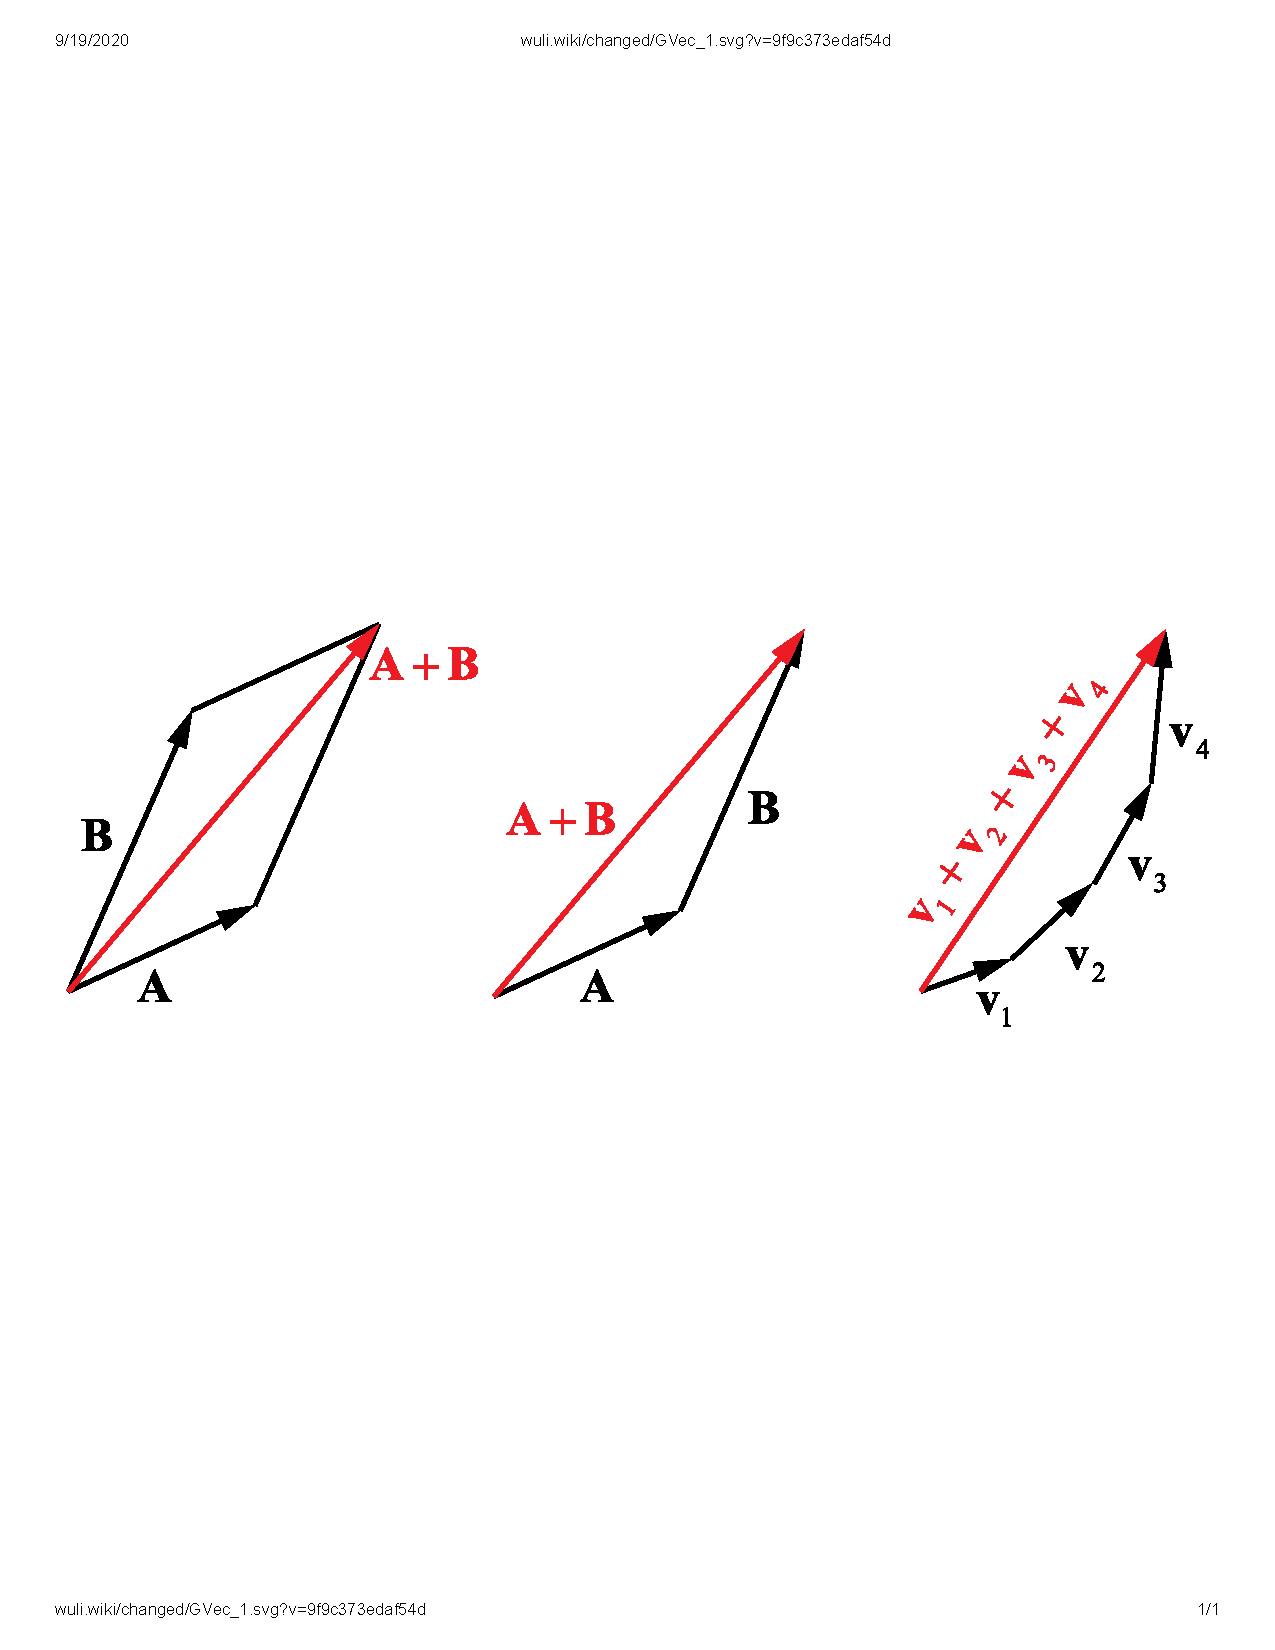
\includegraphics[width=10.5cm]{./figures/GVecOp_1.pdf}
\caption{矢量的加法} \label{GVecOp_fig1}
\end{figure}

\subsubsection{矢量的数乘\ 共线}
第二个矢量运算,是一个矢量和一个数字的乘积,得到一个矢量,称为数乘,我们用例子定义如下.

如\autoref{GVecOp_fig2}, 一个矢量与一个正实数相乘, 则方向不变, 把长度乘以这个实数. 若这个数是负数, 则把矢量取反方向再把长度乘以这个实数数的绝对值即可.若 $\lambda, \mu$ 表示实数, 容易证明分配律 $\lambda(\bvec A + \bvec B) = \lambda\bvec A + \lambda\bvec B$ 和 $(\lambda+\mu)\bvec A = \lambda\bvec A + \mu\bvec A$, 结合律 $\lambda(\mu\bvec A) = (\lambda\mu) \bvec A$.

\begin{figure}[ht]
\centering
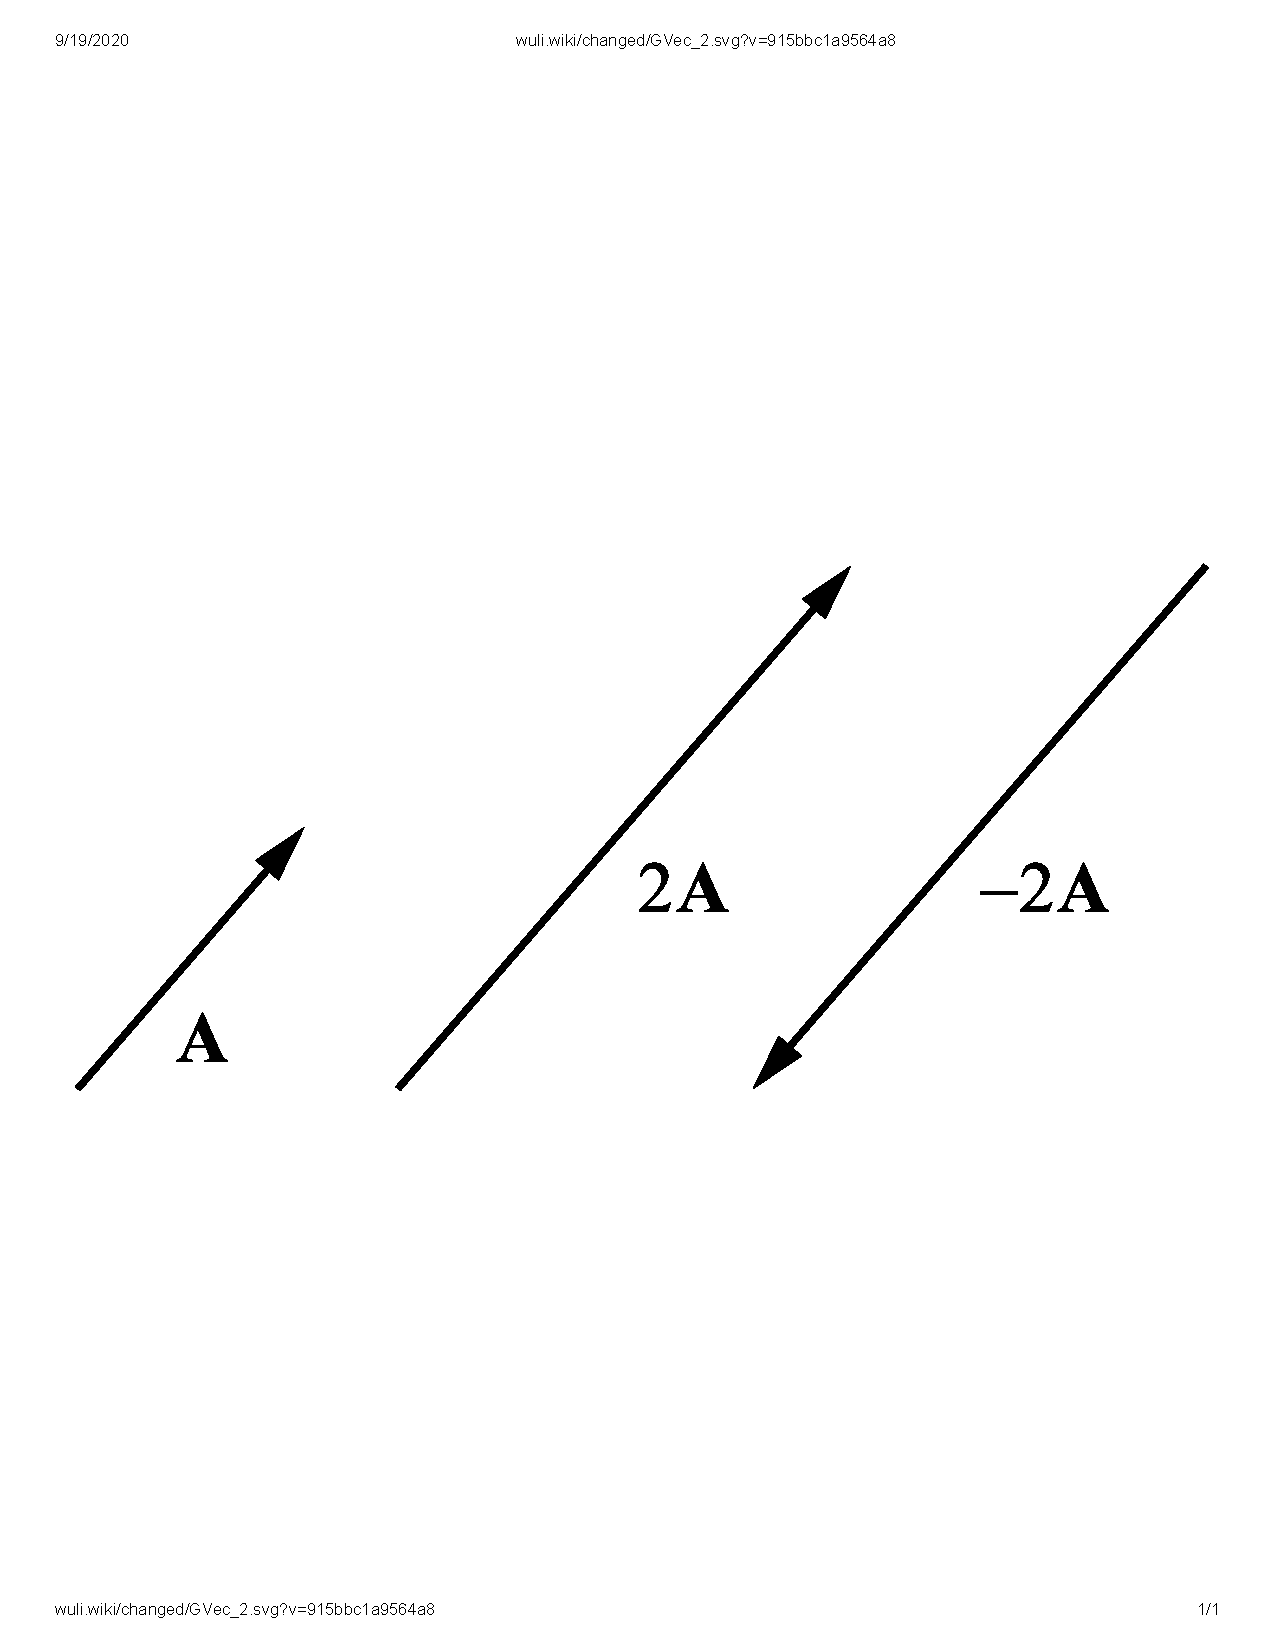
\includegraphics[width=9cm]{./figures/GVecOp_2.pdf}
\caption{矢量的数乘} \label{GVecOp_fig2}
\end{figure}

如果两个矢量的关系可以用 $\bvec A = \lambda\bvec B$ 表示, 那么它们就是\textbf{共线}的. 共线的充分必要条件\upref{SufCnd}是, 两矢量方向相同或相反.

特殊地, 如果把一个矢量乘以 $-1$, 那么它的长度不变, 而方向相反. 我们把这个新矢量叫做原矢量的\textbf{逆矢量(inverse vector)}. 矢量 $\bvec A$ 的逆记为 $-\bvec A$.

\subsubsection{矢量的减法}
由了加法和数乘, 我们并不需要另外定义所谓的\textbf{矢量减法}, 只需要把 $\bvec A - \bvec B$ 看成 $\bvec A$ 加上 $\bvec B$ 的逆即可, 即
\begin{equation}
\bvec A - \bvec B \equiv \bvec A + (-\bvec B)
\end{equation}
几何上来说, 容易证明(留做习题)要计算 $\bvec A - \bvec B$, 就先把它们的起点移动到一起, 然后画出从 $\bvec B$ 的终点指向 $\bvec A$ 的终点的矢量即可.



\subsubsection{移项}
矢量的加减法和我们熟知的标量加减法有许多相似之处, 我们甚至可以像标量移项一样对几何矢量的表达式进行移项. 例如我们有表达式
\begin{equation}
\bvec A + \bvec B = \bvec C + \bvec D
\end{equation}
显然在等式两边同时加上或减去相同的矢量仍然可以使等式成立, 于是两边同时减 $\bvec C$ 再同时减 $\bvec D$ 得
\begin{equation}
\bvec A + \bvec B - \bvec C - \bvec D = \bvec 0
\end{equation}
这看起来就像我们把等号右边得项移动到了等号左边, 并添加了负号.

一个小技巧是, 在画矢量减法 $\bvec A - \bvec B = \bvec C$ 时, 如果你忘记了 $\bvec C$ 是从 $\bvec A$ 指向 $\bvec B$ 还是 $\bvec B$ 指向 $\bvec A$, 那么可以检查一下画出来的三个矢量是否满足 $\bvec A = \bvec B + \bvec C$.


\subsubsection{矢量的线性组合}
把有限个矢量 $\bvec v_i$ 分别与若干实数 $c_i$ 相乘再相加就得到了这些矢量的一个\textbf{线性组合}
\begin{equation}\label{GVecOp_eq1}
\sum_i^N c_i \bvec v_i = c_1\bvec v_1 + c_2\bvec v_2 +\dots +c_N \bvec v_N
\end{equation}

注意,若无特别说明,线性组合仅指\textbf{有限个}矢量的数乘和加法.

根据矢量加法和数乘的定义,容易得知任何有限个矢量的任何线性组合仍然是一个矢量.

\begin{exercise}{}
试说明任意两个不共线的矢量的所有线性组合都会落在同一个平面上.
\end{exercise}

\subsubsection{线性相关性}

如果存在至少一组\textbf{不全为零}系数 $c_i$ 使几个矢量的线性组合等于零, 这些矢量就被称为\textbf{线性相关}的
\begin{equation}\label{GVecOp_eq2}
\sum_i^N c_i \bvec v_i = \bvec 0
\end{equation}
这是因为对于任何一个 $c_j$ 不为零的项, 矢量 $\bvec v_j$ 都可以表示为其他矢量的线性组合. 只需把上式除以 $c_j$ 即可
\begin{equation}\label{GVecOp_eq3}
\bvec v_j = -\sum_{i \ne j}\frac{c_i}{c_j} \bvec v_i
\end{equation}
如果不存在这样的系数, 这些矢量就是\textbf{线性无关}的, 即任何矢量都不可能被其他矢量的线性组合表示. 

\begin{exercise}{}
试说明任意两个共线的矢量必然是线性相关的, 平面任意三个矢量必然是线性相关的.
\end{exercise}

如果一个矢量集合中的矢量是线性相关的,那么这个集合被称为一个\textbf{线性相关组};反之,若线性无关,则称为一个\textbf{线性无关组}.

如果一组矢量之间线性相关,那么至少有一个矢量是“冗余”的,也就是说,它可以被其它矢量的线性组合表示出来.这样一来,对于线性相关的矢量组,如果用它们的线性组合来表示其它矢量,那么表示方式都不是唯一的.线性无关的矢量组,最重要的性质就是它们的线性组合表达式是唯一的,由此引入了基底、坐标等概念.
